%%% DOCUMENT SETUP %%%
\documentclass[11pt,a4paper,onecolumn]{article}
\usepackage[english]{babel}

%%% LAYOUT %%%
\usepackage{fullpage}
\usepackage[a4paper]{geometry}
\usepackage[parfill]{parskip}
\usepackage{multicol}
\usepackage{footnote}

%%% GRAPHICS %%%
\usepackage{graphicx}
\usepackage{color}
\usepackage{graphics}
\usepackage{rotating}
\usepackage{subfig}
\usepackage{amsmath}
\usepackage{amssymb}
\usepackage{amscd}
\usepackage{xfrac}
\usepackage{float}
\usepackage{dsfont}

%%% FONT %%%
\usepackage{ifxetex}
\ifxetex
  \usepackage{fontspec}
    \setmainfont{Linux Libertine O}
  \usepackage{xunicode}
  \usepackage{microtype}
\else
  \usepackage[T1]{fontenc}
  \usepackage[latin1]{inputenc}
  \usepackage{times}
  \usepackage{microtype}
\fi

%%% Coding %%%
\usepackage{listings}
\usepackage{pseudocode}

%%% TITLE PAGE %%%
\author{Jeroen Hofman (10194754) \\
[15pt] University of Amsterdam (\textsc{UvA})}

\title{Concurrent Programming week 2:\\
  Pthreads
		}

\begin{document}
\maketitle
\captionsetup{width=0.8\textwidth}
\lstset{language=Python,breaklines=true,backgroundcolor=\color{white},frame=single}
\thispagestyle{empty}

%%% ABSTRACT %%%
\begin{center}
\begin{abstract}
\small{We investigated a multithreaded version of the sequential code reported last week, and found almost linear performance increase for large matrix sizes up to 8 threads on an 8-core machine. For very large matrices performance is constant for thread numbers bigger than 8 (when the number of threads is a multiple of 8) because the overhead is still negligible for such matrices. For smaller matrices performance declines because of large overhead costs. We also investigated three methods for constructing a barrier and found the mutex/conditionals method the best performing. They have however limited functionality compared to POSIX Pthread functions. Lastly we implemented two versions of the sieve of Eratosthenes, where a version with semaphores is much faster than a version with if-statements.}
\end{abstract}
\end{center}

%%% TABLE OF CONTENTS %%%
\newpage
\tableofcontents
\newpage

\section{Introduction}
Due to the nature of the assignments to be described this week, the setup of the report is different from the previous week. We describe the parallelisation of the code for heat diffusion, barrier implementations in three different ways and two methods to implement an algorithm for the sieve of Eratosthenes. Every problem is described in one section with a subsection describing the algorithm and some technicalities of the code, and a subsection describing results of measurements performed on the code. All measurements in this report are performed with standard compile flags, i.e. -O2.

\section{Heat diffusion with pthreads}
\subsection{Algorithm}
We parallelise the heat diffusion problem from last week using Pthreads (code: /pth/compute.c). We create a number of threads, where every thread is assignment a part of the temperature matrix to compute. Which thread does which part is determined by a small piece of code called the scheduler, which makes sure the load is equally balanced among threads (the difference in workload for threads is at most 1 row). We used only division into blocks along the rows of the matrix, because of locality rules used by the cache. The cache lines of the cache are usually read in the horizontal direction. After scheduling and further initialization of Pthread attributes and other variables, each thread receives an id upon creation which is used to identify the thread and to set appropriate lower and upper bounds for the rows which it has to compute. Each thread also receives a local pointer to the two temperature matrices described in the last report, namely the current temperature matrix and the temperature matrix being computed in the current iteration step. Every thread starts the iterative process by first doing the iteration itself, i.e. filling the assigned rows of the second temperature matrix by doing a computation over the neighbors of the first temperature matrix. During this calculation the threads also compute the maximum difference between the first and second temperature matrix. If the iteration number coincides with some predetermined reporting frequency, every thread will compute its local maximum, minimum and average temperature of its part of the second temperature matrix. After this every thread will proceed (now again regardless of reporting frequency) with copying part of the two halo columns as described in the previous report. After this step the pointers to the temperature arrays are swapped. Note that this can be done independently for every thread, since they use local copies of the pointers to the global arrays. Next the threads will encounter a barrier, they will not go beyond this point before all threads have arrived at this point and hence this is a full synchronization among threads. After all the threads have hit the barrier the master thread (thread with thread id 0) is doing a computation by computing the global maximum difference out of the local maximum difference already computed by every thread (this also explains the use of the first barrier). Depending on the current iteration, it also computes the global maximum, minimum and average temperature from the local values, together with the execution time so far. After this computation the master thread suspends at another barrier. The other threads do not perform this computation but suspend in the second barrier right away. After all threads have hit the second barrier they do the last computation of the iteration step; comparing the threshold value with the global maximum difference computed by the master thread and breaking out of the loop if the global maximum difference is smaller than the threshold. This second barrier has two purposes: Letting the master thread finish the computation of the global maximum difference because it is needed for the threshold condition (for all threads). Secondly it also prevents other threads from already starting the next iteration and hence overwriting local maximum difference values which the master thread needs to compute the global maximum difference (this also holds for the other reporting values, though that only matters when the iteration coincides with the reporting frequency). When the threads break out of the loop, either because of reaching the threshold value or because of reaching the maximum number of iterations, there is a final calculation similar in structure to the intermediate report construction, so local values are computed and the master thread uses these to compute a global value after a barrier is passed.

\subsection{Results}
We test the multithreaded code for different matrix sizes and different number of threads. We set the threshold to zero, the reporting frequency to zero, and the number of iterations to 1000. All measurements are performed on a 8-core node of LISA. The results are given in Table \ref{tab:heat} below. Figure \ref{fig:heat} gives the speedup values with the sequential code as baseline (solid) and the multhithreaded program with one thread as baseline (dashed).

\begin{figure}[H]
  \centering
  \subfloat{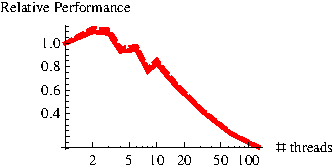
\includegraphics[width=0.33\textwidth]{100.pdf}}
  \subfloat{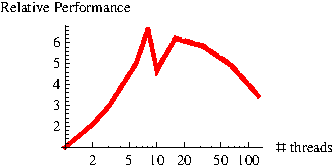
\includegraphics[width=0.33\textwidth]{1000.pdf}}
  \subfloat{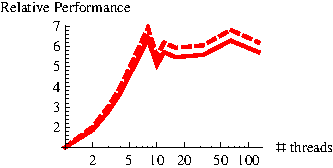
\includegraphics[width=0.33\textwidth]{5000.pdf}}
  \caption{Relative performance results for matrix size 100x100 (left), 1000x1000 (middle) and 5000x5000 (right). The solid line has the sequential code as baseline, the dashed line has the multithreaded code with 1 thread as baseline.}
  \label{fig:heat}
\end{figure}

\begin{table}[H]
  \centering
  \begin{tabular}{l | c | l | c | l }
    \# threads & Execution time & FLOP/s & Execution time & FLOP/s \\
    \hline
    \multicolumn{1}{c}{} & \multicolumn{2}{| c |}{Size 100x100 ($10^6$ iterations)} & \multicolumn{2}{c}{Size 1000x1000}\\
    \hline
    seq. code & 9.159593 & 1.310102 $10^9$ & 16.61579 & 7.222053 $10^8$ \\
    1 & 9.454815 & 1.269195 $10^9$ & 16.75612 & 7.161568 $10^8$ \\
    2 & 8.338178 & 1.439163 $10^9$ & 8.539592 & 1.505221 $10^9$ \\
    3 & 8.443337 & 1.421239 $10^9$ & 5.646020 & 2.125395 $10^9$ \\    
    4 & 9.820339 & 1.221954 $10^9$ & 4.370940 & 2.745407 $10^9$ \\
    6 & 9.681146 & 1.239523 $10^9$ & 3.309898 & 3.625492 $10^9$ \\
    8 & 12.07095 & 9.941227 $10^8$ & 2.496218 & 4.807277 $10^9$ \\
    10 & 10.97233 & 1.093066 $10^9$ &  3.566331 & 3.364806 $10^9$ \\
    12 & 12.19029 & 9.843899 $10^8$ & 3.140024 & 3.821630 $10^9$ \\
    16 & 14.32578 & 8.376510 $10^8$ & 2.527811 & 4.4717194 $10^9$ \\
    32 & 22.31139 & 5.378419 $10^8$ & 2.857517 & 4.199454 $10^9$ \\
    64 & 40.67344 & 2.950329 $10^8$ & 3.372689 & 3.557995 $10^9$ \\
    128 &  83.90564 & 1.430178 $10^8$ & 4.792779 & 2.503769 $10^9$ \\
    \hline
    \multicolumn{1}{c}{} & \multicolumn{2}{| c |}{Size 20000x500} & \multicolumn{2}{c}{Size 500x20000}\\
    \hline
    seq. code & 111.9215 & 1.072181 $10^9$ & 111.8583 & 1.072787 $10^9$ \\
    1 & 116.8893 & 1.026614 $10^9$ & 117.3357 & 1.022708 $10^9$ \\
    2 & 59.85838 & 2.004733 $10^9$ & 59.79632 & 2.006814 $10^9$ \\
    3 & 39.46546 & 3.040636 $10^9$ & 40.02830 & 2.997882 $10^9$ \\
    4 & 30.05528 & 3.992647 $10^9$ & 30.09045 & 3.987980 $10^9$ \\
    6 & 20.96537 & 5.724493 $10^9$ & 21.35896 & 5.618255 $10^9$ \\
    8 & 16.62968 & 7.216018 $10^9$ & 17.73676 & 6.765267 $10^9$ \\
    10 & 24.60525 & 4.877012 $10^9$ & 24.64898 & 4.868359 $10^9$ \\
    12 & 20.78491 & 5.773424 $10^9$ & 21.83848 & 5.494893 $10^9$ \\
    16 & 17.58732 & 6.823102 $10^9$ & 17.54079 & 6.841203 $10^9$ \\
    32 & 17.37267 & 6.907407 $10^9$ & 19.02510 & 6.307461 $10^9$ \\
    64 & 17.40732 & 6.893656 $10^9$ & 18.97766 & 6.323228 $10^9$ \\
    128 & 18.33760 & 6.543937 $10^9$ &  29.74685 & 4.034045 $10^9$ \\
    \hline
    \multicolumn{1}{c}{} & \multicolumn{2}{| c |}{Size 5000x5000} & \multicolumn{2}{c}{}\\
    \hline
    seq. code & 279.1868 & 1.074550 $10^9$ & & \\
    1 & 302.8076 & 9.907289 $10^8$ & & \\
    2 & 149.7098 & 2.003878 $10^9$ & & \\
    3 & 99.12618 & 3.026448 $10^9$ & & \\
    4 & 75.73400 & 3.961236 $10^9$ & & \\
    6 & 53.01261 & 5.659035 $10^9$ & & \\
    8 & 43.62223 & 6.877233 $10^9$ & & \\
    10 & 54.86824 & 5.46764 $10^9$ & & \\
    12 & 48.80707 & 6.146656 $10^9$ & & \\
    16 & 50.89847 & 5.894091 $10^9$ & & \\
    32 & 49.88901 & 6.013354 $10^9$ & & \\
    64 & 44.28577 & 6.774191 $10^9$ & & \\
    128 & 48.73828 & 6.155331 $10^9$ & & \\
  \end{tabular}
  \caption{Results for the multithreaded code for heat diffusion for different matrix sizes and number of threads.}
  \label{tab:heat}
\end{table}

Looking at the matrix size of 100x100, we see that the smallest execution time is achieved for two threads. For larger amount of threads this problem size is too small to give any significant speedup because the overhead costs are too large (the barriers and the master thread specific tasks for instance). If we go to a matrix size of 1000x1000 we observe a speedup however. The speedup up to 8 threads is almost linear in the amount of threads, both with a baseline of the multithreaded program with one thread and the sequential code. This is also what we would expect for 8 cores. The sequential code is slightly faster than the multhithhreaded version with one thread, this difference is caused by the overhead of creating and joining threads. If we look at the behavior of execution time beyond 8 threads, we see a worse performance first but at 16 threads there is again a minimum in the execution time. This minimum is slightly higher than for 8 threads. The decrease in performance at 10 and 12 cores is caused by the amount of threads being not a multiple of the amount of available cores. This causes some 'leftover' threads which have to be scheduled whenever one of the cores is not occupied. This situation becomes better at 16 threads, where every core most likely has two threads and no much rescheduling is needed. However, 2 threads on one core is less efficient still than 1 thread per core, hence the slightly worse performance. If we look at 32, 64 and 128 threads we observe that execution times are still decent because they are all multiple of 8, with performance decreasing slightly for increasing thread number, which is caused by overhead. If the number of threads per core increases, the scheduler has to perform more and more rescheduling, damaging performance.

If we look at the performance measurements for matrix sizes 500x20000 and 20000x500 we see that they almost perform the same for low number of threads. Maximal performance is again achieved at 8 threads, decreasing for 10 and 12 threads and increasing again for 16 threads. After 16 threads the performance stays constant, this is probably caused by the size of the matrix, which causes the overhead produced by the scheduler of the processors etc. to still be negligible (except for 128 threads). The computation time (the iteration itself) is most likely still the dominant factor. There are significant performance differences between the two matrix sizes for 6, 8, 32, 64 and 128 threads, this is caused by an uneven workload for the matrix of size 500x20000 since 6, 8 32, 64 and 128 are not divisors of 500, they are however divisors of 20000. Due to the vertical (row) block scheduling used this effect is visible in performance measurements. This effect is enhanced because the rows for the 500x20000 matrix are very large.

Lastly we look at the matrix of size 5000x5000. This matrix has roughly the same behavior as the matrices of size 20000x500 and 500x20000, with also a plateau in performance at 16, 32 and 64 threads. This is mostly likely again caused by a still negligible overhead. The performance for 12 cores is remarkably good, unlike the other matrix sizes. A possible explanation might be the hyper threading that is present on the LISA 8 cores, which causes maybe some cache relocation or has some other performance increasing attributes (I did not look into this). 

To conclude, overall we see almost linearly increasing performance for increasing number of threads up to 8 threads, with a maximum performance at 8 threads, and a second slightly lower maximum at 16 threads, except for very large matrix sizes where the performance stays constant or even increases after 8 threads, most likely since the overhead is still negligible. 

\section{Barrier synchronization}
In this section we look at three different structures for barriers. A barrier in the thread context is a structure which synchronizes all or part of the threads. Threads arriving at the barrier are suspended until a sufficient number of threads has reached the barrier, at that point all the suspended threads are waken up and can continue with executing their code. We will look at three different structures; the original POSIX Pthread implementation using the functions \texttt{pthread\_barrier\_init} and \texttt{pthread\_barrier\_wait}, an implementation using semaphores and an implementation using Pthread mutex locks and condition variables.

\subsection{The original POSIX functions}
This code can be found in /pth/assignment\_2.3/original.c . It is a very simple setup where a number of Pthreads are created and repeatedly call a barrier in a loop. The calling function has an argument which is usually equal to the number of threads, meaning that threads are only waken up from suspension when all threads have hit the barrier. 

\subsection{Mutex locks and condition variables}
This code can be found in /pth/assignment\_2.3/mutex.c . This code implements a barrier using only the \texttt{pthread\_mutex\_t} and \texttt{pthread\_cond\_t} data types. The code that will be discussed is taken from Ref. \cite{mutex}, which was found during a search on the internet for more information on internal barrier handling by pthreads. The code creates a type \texttt{struct barrier\_t} containing two integers called \emph{max} and \emph{number}, a mutex lock and a condition. The function \texttt{mythread\_barrier\_init} initializes the lock and the condition variables, and sets \emph{max} to some number which is usually equal to the number of threads (but certainly not larger) and \emph{number} to 0. The function \texttt{mythread\_barrier\_wait} is repeatedly called by the threads in a loop. A thread arriving at this function obtains first a lock, then \emph{number} is increased. If \emph{number} is not equal to \emph{max}, the thread is suspended using \texttt{pthread\_cond\_wait}, which releases the lock (actually not the lock itself, but a copy of it). More threads will arrive and get suspended with \texttt{pthread\_cond\_wait} until \emph{number} is equal to \emph{max}, then \emph{number} is set to zero and the thread calls \texttt{pthread\_cond\_broadcast}, which wakes up all the threads, which will then execute the rest of the function which consists of unlocking the lock. This is a simple construction which is very fast to implement, as we will see later. In fact, it could be that the original POSIX functions \texttt{pthread\_barrier\_wait} and \texttt{pthread\_barrier\_init} use locks and condition variables in the same way as described before.

\subsection{Semaphores}
This code can be found in /pth/assigment\_2.3/sema.c . The code mimics a barrier using only the concept of semaphores. A semaphore is effectively a counter which can be incremented (\texttt{sem\_post}) and decremented (\texttt{sem\_wait}) with the special property that a decrement cannot lead to values beneath zero. The thread suspends if this happens until some other thread does a \texttt{sem\_post} and the value can be decremented again. This code is inspired on Ref. \cite{sema}, which is a very useful book of one wants to learn something about semaphores. The solution to this problem is spelled out in the book, but it also gives hints before giving the solution. I actually only used the hints provided in the book (not the solution!) after creating three different semaphore structures myself, which all contained (on a deep level) race conditions. The race conditions I usually got were that a thread was able to go twice through the function unharmed which would be incorrect since it would set off the timer twice and hence other threads would not have to reach the barrier before the other threads are released again. This could be fixed by putting a lock around the whole code, effectively slowing down the code since everything is done sequentially. The hint in the book said it would be wise to implement two sections, one for arrival and one for departure and with this hint I was able to solve the problem.
 
We again have a struct mimicking a barrier containing three semaphores (all having the function of a lock) and two integers, \emph{add} initialized to 0 and \emph{maxCount} initialized to some number, usually equal to the number of threads. Threads calling \texttt{mythread\_barrier\_wait} obtain the first lock and increment \emph{add}, the first lock is released again and they call another second lock, which is initialized to zero and so the threads suspend. The last thread obtaining the first lock decrements a third lock and increments the second lock. Now all the threads are waken up again and they go through the second lock (by decrementing and incrementing the semaphore value of the second lock). They then enter exactly the same structure, they obtain the first lock again, but now decrement the value of \emph{add} and now they get suspended at the third lock (which was set to zero when the last thread entered the first construction). This again goes on until the last thread obtains the first lock and enters the second structure. This thread sets the second lock to zero and sets the third lock to one, so all the threads wake up and they can call \texttt{mythread\_barrier\_wait} again for the next loop. There are no race conditions here since the last thread arriving at one of the construction sets a lock at the end of the next one and then releases the lock at which all the other threads are waiting. Though this structure works, it is not very fast, because of the three locks and the extra 'barrier' in the middle of the code between the two constructions.

\subsection{Results}
We measured the total execution time of initializing the barriers, creating the threads and executing the function which calls \texttt{mythread\_barrier\_wait} in a loop of 800.000 iterations. The results are given in Table \ref{tab:barrier} below. The results are generated on a LISA node with 8 cores.

\begin{table}[H]
  \centering
  \begin{tabular}{l | c | c}
  Number of threads  & Total execution time & Execution time per iteration \\
  \hline
  \multicolumn{3}{c}{Semaphore barrier}\\
  \hline
  1 & 0.160773 & < 0.000001 \\
  2 & 14.964482 & 0.000019 \\
  4 & 22.435938 & 0.000028 \\
  8 & 51.923563 & 0.000065 \\
  \hline
  \multicolumn{3}{c}{POSIX functions} \\
  \hline
  1 & 0.151738 & < 0.000001 \\
  2 & 3.524765 & 0.000004 \\
  4 & 22.070229 & 0.000028 \\
  8 & 51.247505 & 0.000064 \\
  \hline
  \multicolumn{3}{c}{Mutex locks and condition variables} \\
  \hline
  1 & 0.054546 & < 0.000001 \\
  2 & 5.962033 & 0.000007 \\
  4 & 17.599998 & 0.000022 \\
  8 & 35.319528 & 0.000044 \\
  \end{tabular}
  \caption{Execution times for 800.000 iterations for three different barrier calls and different numbers of threads.}
  \label{tab:barrier}
\end{table}

The worst performance is given by the semaphore implementation. This implementation gives nearly the same results as the original POSIX functions but is slower for 2 threads. Since one mostly encounters applications with four or more threads, the best implementation in this case is the one with mutex locks and condition variables. A possible explanation why this is faster might be that the original POSIX functions do the same, only they can also accept certain attributes (set to NULL in both the semaphore and mutex implementation) and have to do more exception and error handling. In this case the comparison might not really be fair, since the POSIX functions have more added functionality.

\section{Sieve of Eratosthenes}
\subsection{Algorithm}
In this section we describe an implementation of the sieve of Eratosthenes using Pthreads. We will first describe the general algorithm and then go into the details of the code (to be found in /pth/assignment\_2.4/sieve\_slow.c). The general algorithm is very simple, one starts with the integer 2 which acts like a filter and then considers subsequent integers. If the integer considered is not a multiple of two, it passes the filter and if the integer is not a filter itself yet, it becomes one. So for instance 3 will pass the filter and become a filter, 4 will be filtered out by 2, 5 will pass through the filters 2 and 3 and become a filter itself. In this way all the filters will correspond to a prime number. Though this algorithm is far from efficient since for large numbers the amount of filters becomes very large, it is an algorithm well suited for implementation of a pipeline of threads.

This is also what happens when we look at the code. We first create a generator thread, which simply generators integers starting from 2 and stores them in a bounded buffer of some size (\emph{BUFSIZE} in the code). We then create a thread which is associated with the number 2, it reads numbers from the buffer which are stored there by the generator and it stores numbers on its own buffer, again with size \emph{BUFSIZE}. This filter (and subsequently created filters) loop through a piece of code until a fixed number of primes is found, then the thread terminates. The piece of code consists of a few pieces: first the filter thread checks if there is something in the buffer from the previous filter (or the generator in the case of the filter for 2) and it also checks if there is space in its own buffer. If these conditions are met the number received from the buffer of the previous filter or generator is considered a candidate to be prime and tested. If the thread filter number divides the candidate this number is discarded and the thread will look at the next space in the buffer of the previous filter/generator and repeat. If the candidate however is not a divisor of the filter thread number, one out of two things can happen. If the current thread is the last thread in the pipeline it will create a new thread with the the thread filter number equal to the candidate, else it will put the candidate in its own buffer, ready to be read by the next filter thread.

There are some drawbacks and advantages to the the code is set up. One of the drawbacks is the double if- condition in the beginning, since this is a strict condition (the thread has to have space to put its candidate and there must be a number to process) a big portion of time the threads will end up going through the while loop without actually doing anything. On the other hand, there is no need for locks with this set-up since no race conditions can occur. The only race condition that could occur is by assigning a thread\_id when a new candidate is found and no subsequent filter is present, but since only one of the threads can be in this situation, this race condition never occurs. I have tried putting one or both of the out most if-conditions more inside, but either the primes are reported but end up scrambled, or primes are skipped because numbers are being overwritten in the buffers.

Due to the nature of the problem the execution time is large and gets larger for larger number of primes to be found for two reasons: there are more threads running so more overhead in creating and joining and general scheduling, and also it takes numbers longer to go through all the filters. This could be made more efficient by for instance excluding in advance all multiples of 1...10 in the generator, this is easy to check and would results in much less junk getting sent into the pipeline, for instance all the even numbers.

It is worth mentioning that there is a very strange bug in the code regarding the termination of threads. In the code there is a do-while loop which was originally a while-loop. This works fine although when the threads should terminate some of them (randomly) do not terminate and the main thread never closes properly. After experimenting the following was found:
\begin{itemize}
\item 
  It works with a do-while loop instead of a while-loop
\item
  It works with a while-loop with some random printf statement put somewhere in the loop.
\item
  It works with a while-loop without -O2 optimization (which is the standard compiler flag in the skeleton)
\end{itemize}
This indicates that something may go wrong in the compilation of the problem with -O2, something is probably executed too fast which locks some of the threads. The printf would then delay things (because it is an expensive operation) which would fix the bug. I have not been able to identify what is going wrong precisely and probably one has to dive into Assembly to find it out.

I decided to make another version of the sieve, this time using semaphores (/pth/assignment\_2.4/sieve\_fast.c). The structure is similar to the structure of the code described above, only this time we use semaphores instead of the double if statement mentioned before. There are two semaphores per buffer, one denoting the number of free spaces and one denoting the number of occupied spaces in the buffer of size \emph{BUFSIZE}. A thread waits until there is something put in the previous buffer, then it takes it and it decrements the semaphore value representing the occupation of that buffer. It then signals to the previous buffer that it has taken something, increasing the available space in that buffer, this is done by incrementing the semaphore representing the number of free spaces. The reason that this cannot be done with one semaphore is that the thread needs time to write the value found in the buffer to its own local variable. To summarize:
\begin{itemize}
\item 
  The thread waits until the buffer is not empty.
\item
  The thread decrements the semaphore value of the occupation.
\item
  The thread writes the value of the buffer to a local variable.
\item
  The thread increments the semaphore value of the empty spaces, signalling there is room for more values now.
\end{itemize}
Then the candidate value is checked whether or not it divides the prime number associated with the thread. When it does not divide we again either create a new thread with the current thread, or we put the value in the current buffer, by a similar method as described above, the thread waits for an empty space, then writes to the buffer, than signals the next thread that there is something in the buffer by incrementing the semaphore value for the occupation.
This method is much, much faster than the other one, as we will see below. There is however a problem with this method, if all the desired primes are found, the threads are supposed to terminate. However, some of the threads might be suspended by a \texttt{sem\_wait} function, waiting either until they can get a new value from the buffer of the previous thread, or waiting to put a new candidate in their buffer. To circumvent this, the last thread that is created will increment all semaphore values of all buffers, thereby forcing all the threads to finish their iteration and recheck the condition of the do-while loop, and hence terminate since the condition is no longer satisfied.

\subsection{Results}
We have done some small test with 2 different buffer sizes and prime numbers, between the two programs. The results are shown in Table \ref{tab:sieve} below. All measurements are performed on the LISA home node.
\begin{table}[H]
  \centering
  \begin{tabular}{l | c}
    \hline
    \multicolumn{2}{c}{Sieve with double-if statement}\\
    \hline
    BUFSIZE = 10, primes = 100 & 3.12 \\
    BUFSIZE = 100, primes = 100 & 2.83 \\
    BUFSIZE = 10, primes = 1000 & > 100 \\
    BUFSIZE = 100, primes = 1000 & > 100 \\
    \hline
    \multicolumn{2}{c}{Sieve with semaphores}\\
    \hline
    BUFSIZE = 10, primes = 100 &  0.01 \\
    BUFSIZE = 100, primes = 100 & 0.01 \\
    BUFSIZE = 10, primes = 1000 & 0.37 \\
    BUFSIZE = 100, primes = 1000 & 0.19 \\
  \end{tabular}
  \caption{Performance of two implementations of the sieve of Eratosthenes. The execution times reported are the minima over 10 runs.}
  \label{tab:sieve}
\end{table}

There is a large fluctuation between runs on LISA, the reason being that there are many threads and the way the processor(s) schedule the threads is random, so one run the scheduling might be much more optimal than another time, this is a general feature of pipeline processes like the sieve. It is clear from the table that the second version is much better than the first one, hence this version will be the standard compiled version when executing \texttt{make}. The influence of the buffer size is not really clear but higher buffer sizes might increase performance because the threads have more work when they wake up, this will prevent a thread from going into suspension mode again after a very short time.

\section{Conclusions}
We investigated performance of a piece of multithreaded code for heat diffusion. We found significant linear speedups with the best performance at 8 threads on an 8-core machine. Depending on the matrix size either the performance declines after 8 threads due to increased overhead, or performance stays more or less the same because computation is still orders of magnitude more time consuming than overhead. Thread numbers above 8 which are not a multiple of 8 cause significant decrease in performance. 
We also investigated three different ways to implement a barrier for threads. Of all three implementations the mutex lock and condition variables method was most time-efficient. However, since these implementations are very simple, they are not fairly compared with the original POSIX Pthread functions, which have more added functionality.
Lastly we build two versions of the sieve of Eratosthenes, one using only if-statements, another using semaphores. The semaphore solution turned out to be significantly faster to generate a fixed number of primes. Also increasing buffer size may increase performance, though the results are not very clear.

%%% BIBLIOGRAPHY %%%
\begin{thebibliography}{7}
\bibitem{LISA}
  http://sara.nl/systems/lisa/description
\bibitem{mutex}
  http://www.howforge.com/implementing-barrier-in-pthreads
\bibitem{sema}
  A.B. Downey, \emph{The Little Book of Semaphores}, 2008, version 2.1.5
\end{thebibliography}

\end{document}
